\subsection{Experiment 2: Accelerating Convergence through Elevated Learning Rates} \label{sec:exp2}

Given the extended convergence observed during the initial experiment, the author deliberated on a strategic approach to hasten the convergence rate. This led to the contemplation of raising the learning rates as a feasible method of accelerating the convergence process.

This model shared the same number of parameters (about 4 million), loss function (\ac{BCE}), dataset, optimizer, and hardware setup as the former one.

The learning rate, for both the generator and the discriminator, was elevated to $1 \times 10^{-2}$. At the conclusion of the training process, the generator’s loss was calculated at $0.545$, and the discriminator’s loss was measured at $1.412$. The total loss, represented as the cumulative sum of the generator and discriminator losses, was calculated at $1.957$.

Upon evaluation, the spectrogram of the initial model was determined to be similar to the first one. The point at which the models began learning at a slower rate was reached more quickly, but the outcomes remained unsatisfactory.

Figure~\ref{fig:exp2_results} shows the loss and final spectrogram produced.

\begin{figure}[!ht]
    \centering
    \begin{subfigure}{0.45\textwidth}
        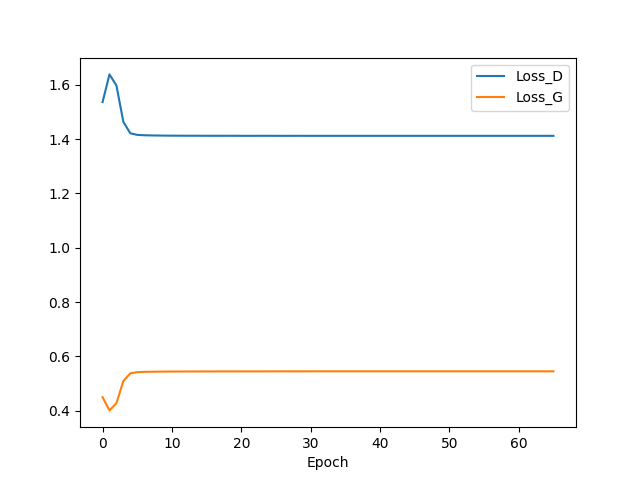
\includegraphics[width=\textwidth]{figures/4.5-results/exp2_loss.png}
        \caption{Evolving losses throughout the training process for Experiment 2.}
        \label{fig:exp2_loss}
    \end{subfigure}
    \begin{subfigure}{0.45\textwidth}
        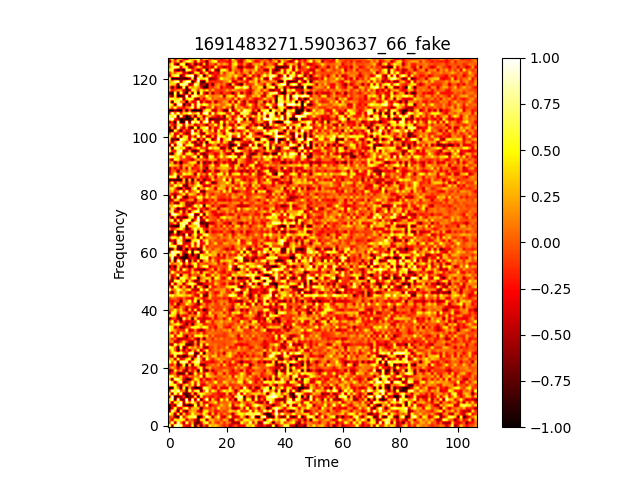
\includegraphics[width=\textwidth]{figures/4.5-results/exp2_spectrogram.png}
        \caption{Spectrogram generated in Experiment 2.}
        \label{fig:exp2_spectrogram}
    \end{subfigure}
    \caption{Results of Experiment 2.}
    \label{fig:exp2_results}
\end{figure}